\documentclass{osa-article}

%% Select the journal you're submitting to
%% oe, boe, ome, osac, osajournal
\journal{osajournal}
% Key:
% Express journals must have the correct journal selected:
% {oe} Optics Express
% {boe} Biomedical Optics Express
% {ome} Optical Material Express
% {osac} OSAC Continuum
% Other OSA journals may use:
% {osajournal} Applied Optics, Advances in Optics and Photonics, Journal of the Optical Society of America A/B, Optics Letters, Optica, Photonics Research

% Uncomment if submitting to Photonics Research.
% ONLY APPLICABLE FOR \journal{osajournal}
% \setprjcopyright

% Set the article type
\articletype{Research Article}
% Note that article type is not required for Express journals (OE, BOE, OME and OSAC)

\begin{document}

\title{Frame Localisation Optical Projection Tomography}

\author{Craig Russell,\authormark{1*,2} Eric Rees,\authormark{1}}

\address{\authormark{1}\\
\authormark{2}\\
\authormark{3}}

\email{\authormark{*}craig.russell@npl.co.uk} %% email address is required

% \homepage{http:...} %% author's URL, if desired

%%%%%%%%%%%%%%%%%%% abstract %%%%%%%%%%%%%%%%
%% [use \begin{abstract*}...\end{abstract*} if exempt from copyright]

\begin{abstract}
\LaTeX{} manuscripts submitted to OSA journals as of 30 May 2018 may use these instructions and this new single-column universal template format. Note that the final publishing format of OSA journals is not changing at this time, and authors will still need to adhere to article-length restrictions based on the final publishing format (which for some journals is two columns). Authors of Optics Letters articles and Optica letters and memoranda should continue using the legacy template for an accurate length check. Please note that OSA is no longer using OCIS codes.
\end{abstract}

%%%%%%%%%%%%%%%%%%%%%%%%%%  body  %%%%%%%%%%%%%%%%%%%%%%%%%%
\section{Introduction}
Adherence to the specifications listed in this template is essential for efficient review and publication of submissions. Proper reference format is especially important (see Section \ref{sec:refs}).

\section{Multiple corresponding authors}

There are two options for indicating multiple corresponding authorship, and they are formatted quite differently. The first format would be as follows and uses an asterisk to denote one of the authors:

\begin{verbatim}
\author{Author One\authormark{1,3} and Author Two\authormark{2,4,*}}

\address{\authormark{1}Peer Review, Publications Department,
Optical Society of America, 2010 Massachusetts Avenue NW,
Washington, DC 20036, USA\\
\authormark{2}Publications Department, Optical Society of America,
2010 Massachusetts Avenue NW, Washington, DC 20036, USA\\
\authormark{3}xyz@osa.org}

\email{\authormark{*}opex@osa.org}
\end{verbatim}

This format will generate the following appearance:

\medskip

\author{Author One\authormark{1,3} and Author Two\authormark{2,4,*}}

\address{\authormark{1}Peer Review, Publications Department,
Optical Society of America, 2010 Massachusetts Avenue NW,
Washington, DC 20036, USA\\
\authormark{2}Publications Department, Optical Society of America,
2010 Massachusetts Avenue NW, Washington, DC 20036, USA\\
\authormark{3}xyz@osa.org}

\email{\authormark{*}opex@osa.org}

\medskip

The second format forgoes the asterisk and sets all email addresses equally within the affiliations. Please note that this format does not use the \verb+\email{}+ field at all.
\begin{verbatim}
\author{Author One\authormark{1,3} and Author Two\authormark{2,4}}

\address{\authormark{1}Peer Review, Publications Department,
Optical Society of America, 2010 Massachusetts Avenue NW,
Washington, DC 20036, USA\\
\authormark{2}Publications Department, Optical Society of America,
2010 Massachusetts Avenue NW, Washington, DC 20036, USA\\
\authormark{3}xyz@osa.org\\
\authormark{4}opex@osa.org}
\end{verbatim}

This format will generate the following appearance:

\medskip

\author{Author One\authormark{1,3} and Author Two\authormark{2,4}}

\address{\authormark{1}Peer Review, Publications Department,
Optical Society of America, 2010 Massachusetts Avenue NW, Washington, DC 20036, USA\\
\authormark{2}Publications Department, Optical Society of America, 2010 Massachusetts Avenue NW, Washington, DC 20036, USA\\
\authormark{3}xyz@osa.org\\
\authormark{4}opex@osa.org}
\medskip
These are the preferred
%express journal
formats for multiple corresponding authorship, and either may be used.

\section{Abstract}
The abstract should be limited to approximately 100 words.
%It should be an explicit summary of the paper that states the problem, the methods used, and the major results and conclusions. It also should contain the relevant key words that would allow it to be found in a cursory computerized search.
If the work of another author is cited in the abstract, that citation should be written out without a number, (e.g., journal, volume, first page, and year in square brackets [Opt. Express {\bfseries 22}, 1234 (2014)]), and a separate citation should be included in the body of the text. The first reference cited in the main text must be [1]. Do not include numbers, bullets, or lists inside the abstract.

\begin{figure}[h!]
\centering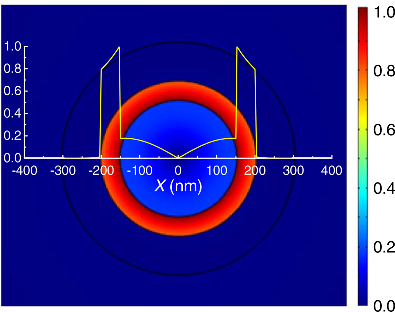
\includegraphics[width=7cm]{osafig1}
\caption{Sample caption (Fig. 2, \cite{Yelin:03}).}
\end{figure}


\section{Assessing final manuscript length}
OSA's Universal Manuscript Template is based on the OSA Express layout and will provide an accurate length estimate for Optics Express, Biomedical Optics Express,  Optical Materials Express, and OSA's newest title OSA Continuum. Applied Optics, JOSAA, JOSAB, Optics Letters, Optica, and Photonics Research publish articles in a two-column layout. To estimate the final page count in a two-column layout, multiply the manuscript page count (in increments of 1/4 page) by 60\%. For example, 11.5 pages in the OSA Universal Manuscript Template are roughly equivalent to 7 composed two-column pages. Note that the estimate is only an approximation, as treatment of figure sizing, equation display, and other aspects can vary greatly across manuscripts. Authors of Letters may use the legacy template for a more accurate length estimate.

\section{Figures, tables, and supplemental materials}

\subsection{Figures and tables}

OSA encourages authors to submit color figures with their manuscripts. Figures and tables should be placed in the body of the manuscript. Standard \LaTeX{} environments should be used to place tables and figures:
\begin{verbatim}
\begin{figure}[htbp]
\centering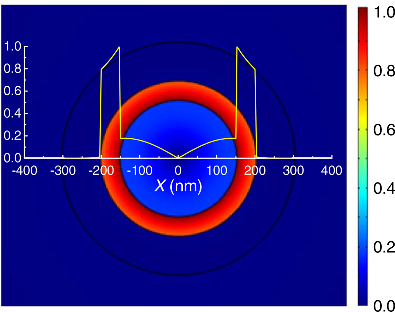
\includegraphics[width=7cm]{osafig1}
\caption{Sample caption (Fig. 2, \cite{Yelin:03}).}
\end{figure}
\end{verbatim}

\subsection{Supplementary materials in OSA journals}

OSA journals allow authors to include supplementary materials as integral parts of a manuscript. Such materials are subject to peer-review procedures along with the rest of the paper and should be uploaded and described using OSA's Prism manuscript system. Please see the \href{http://www.osapublishing.org/submit/style/multimedia.cfm}{Author Guidelines for Supplementary Materials in OSA Journals} for further information.

Supplementary materials must be associated with a figure, table, or equation, OR be referenced in the results section of the manuscript. Please note that to create text color for supplementary materials links, use of the command \\
\verb|\textcolor{urlblue}{Visualization 1}| is preferred to using the command\\
\verb|\url{Visualization 1}|.

\begin{figure}[ht!]
\centering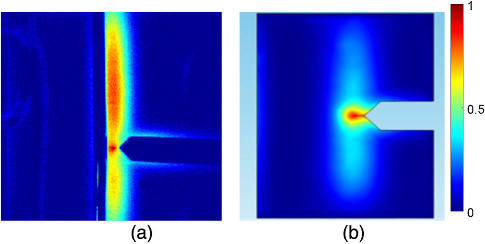
\includegraphics{osafig2}
\caption{(a) Three traps create three rings of magnetic nanoparticles. (b) The rings interact with one another (see \textcolor{urlblue}{Visualization 1}, \cite{Masajada:13}).}
\end{figure}


\begin{verbatim}
\begin{figure}[hbt!]
\centering\includegraphics{opexfig2}
\caption{Normalized modulus distributions of transverse electrical
field components of the TM01 mode in PWs with (a) SiO_2 core
and (b) Si core}{Visualization 1}), \cite{Masajada:13}).}
\end{figure}
\end{verbatim}

\section{Mathematical and scientific notation}

\subsection{Displayed equations} Displayed equations should be centered.
Equation numbers should appear at the right-hand margin, in
parentheses:
\begin{equation}
J(\rho) =
 \frac{\gamma^2}{2} \; \sum_{k({\rm even}) = -\infty}^{\infty}
	\frac{(1 + k \tau)}{ \left[ (1 + k \tau)^2 + (\gamma  \rho)^2  \right]^{3/2} }.
\end{equation}

All equations should be numbered in the order in which they appear
and should be referenced  from within the main text as Eq. (1),
Eq. (2), and so on [or as inequality (1), etc., as appropriate].


\section*{Funding}
Please identify all appropriate funding sources by name and contract number. Funding information should be listed in a separate block preceding any acknowledgments. List only the funding agencies and any associated grants or project numbers, as shown in the example below:\\
\\
National Science Foundation (NSF) (1253236, 0868895, 1222301); Program 973 (2014AA014402); Natural National Science Foundation (NSFC) (123456).\\
\\
OSA participates in \href{https://www.crossref.org/fundingdata/}{Crossref's Funding Data}, a service that provides a standard way to report funding sources for published scholarly research. To ensure consistency, please enter any funding agencies and contract numbers from the Funding section in Prism during submission or revisions.

\section*{Acknowledgments}
Acknowledgments, if included, should appear at the end of the document. The section title should not be numbered.

\section*{Disclosures}
For \textit{Biomedical Optics Express} submissions only, disclosures should be listed in a separate nonnumbered section at the end of the manuscript. List the Disclosures codes identified on OSA's \href{http://www.osapublishing.org/submit/review/conflicts-interest-policy.cfm}{Conflict of Interest policy page}, as shown in the examples below:\\
\\
ABC: 123 Corporation (I,E,P), DEF: 456 Corporation (R,S). GHI: 789 Corporation (C).\\
\\
If there are no disclosures, then list ``The authors declare that there are no conflicts of interest related to this article.''


\section{References}
\label{sec:refs}
Proper formatting of references is extremely important, not only for consistent appearance but also for accurate electronic tagging. Please follow the guidelines provided below on formatting, callouts, and use of Bib\TeX.

\subsection{Formatting reference items}
Each source must have its own reference number. Footnotes (notes at the bottom of text pages) are not used in OSA journals. References require all author names, full titles, and inclusive pagination. Examples of common reference types can be found on the  \href{http://www.osapublishing.org/submit/style/style_traditional_journals.cfm} {Author and Reviewer Resource Center}.


The commands \verb+\begin{thebibliography}{}+ and \verb+\end{thebibliography}+ format the section according to standard style, showing the title {\bfseries References}.  Use the \verb+\bibitem{label}+ command to start each reference.

\subsection{Formatting reference citations}
References should be numbered consecutively in the order in which they are referenced in the body of the paper. Set reference callouts with standard \verb+\cite{}+ command or set manually inside square brackets [1].

To reference multiple articles at once, simply use a comma to separate the reference labels, e.g. \verb+\cite{Yelin:03,Masajada:13,Zhang:14}+, produces \cite{Yelin:03,Masajada:13,Zhang:14}.
%Using the \texttt{cite.sty} package will make these citations appear like so: [2--4].

\subsection{Bib\TeX}
\label{sec:bibtex}
Bib\TeX{} may be used to create a file containing the references, whose contents (i.e., contents of \texttt{.bbl} file) can then be pasted into the bibliography section of the \texttt{.tex} file. A Bib\TeX{} style file, \texttt{osajnl.bst}, is provided.

\section{Conclusion}
After proofreading the manuscript, compress your .tex manuscript file and all figures (which should be in EPS or PDF format) in a ZIP, TAR or TAR-GZIP package. All files must be referenced at the root level (e.g., file \texttt{figure-1.eps}, not \texttt{/myfigs/figure-1.eps}). If there are supplementary materials, the associated files should not be included in your manuscript archive but be uploaded separately through the Prism interface.

%%%%%%%%%%%%%%%%%%%%%%% References %%%%%%%%%%%%%%%%%%%%%%%%%

Add references with BibTeX or manually.
\cite{Zhang:14,OSA,FORSTER2007,Dean2006}

%%%%%%%%%% If using BibTeX:
\bibliography{sample}

%%%%%%%%%% If preparing manually:
% \begin{thebibliography}{1}
% \newcommand{\enquote}[1]{``#1''}

% \bibitem{Zhang:14}
% Y.~Zhang, S.~Qiao, L.~Sun, Q.~W. Shi, W.~Huang, L.~Li, and Z.~Yang,
%   \enquote{Photoinduced active terahertz metamaterials with nanostructured
%   vanadium dioxide film deposited by sol-gel method,}
%   {\protect\JournalTitle{Optics Express}} \textbf{22}, 11070--11078 (2014).

% \bibitem{OSA}
% {Optical Society}, \enquote{{OSA Publishing},}
%   \url{http://www.osapublishing.org}.

% \bibitem{FORSTER2007}
% P.~Forster, V.~Ramaswamy, P.~Artaxo, T.~Bernsten, R.~Betts, D.~Fahey,
%   J.~Haywood, J.~Lean, D.~Lowe, G.~Myhre, J.~Nganga, R.~Prinn, G.~Raga,
%   M.~Schulz, and R.~V. Dorland, \enquote{Changes in atmospheric consituents and
%   in radiative forcing,} in \enquote{Climate Change 2007: The Physical Science
%   Basis. Contribution of Working Group 1 to the Fourth assesment report of
%   Intergovernmental Panel on Climate Change,}  S.~Solomon, D.~Qin, M.~Manning,
%   Z.~Chen, M.~Marquis, K.~B. Averyt, M.~Tignor, and H.~L. Miler, eds.
%   (Cambridge University Press, 2007).

% \end{thebibliography}


\end{document}
